\chapter{Sistema de grabación online}

Para poder obtener grabaciones de distintas personas se desarrolló una página web. Esto es muy conveniente ya que nos permite grabar fácilmente desde cualquier lugar. En esta sección explicaremos la arquitectura del sistema y sus detalles técnicos.

La página web está desarrollada en Django, versión 1.4.2. Se eligió este framework por su facilidad a la hora de guardar objetos a la base de datos y también por la cantidad importante de bibliotecas que posee Python. La versión de Python que se utilizó es 2.7.3. 

En la base de datos se guarda la información de cada hablante, las frases a grabar y las trazas. La base de datos elegida fue PostgreSQL versión 9.1 y se escogió ésta ya que es de código abierto entre otras cosas. Los audios se guardan en archivos \textit{wav} por separado y también se guarda una referencia al nombre del archivo generado en la base de datos. Para el servidor HTTP se utiliza Apache versión 2.2.22. El servidor utiliza el sistema operativo Ubuntu 12.04.4 LTS.

\section{Recolección de datos}

Cuando un usuario visita nuestra página, primero debe llenar un formulario. Este le pregunta: género, fecha de nacimiento, lugar donde se crió y donde reside actualmente. Al confirmar el formulario, los datos son grabados en la base de datos en el servidor. Esto se puede apreciar en la Figura \ref{figEncuesta}. Luego se procede a realizar las grabaciones. 

\begin{figure}[h!]
    \centerline{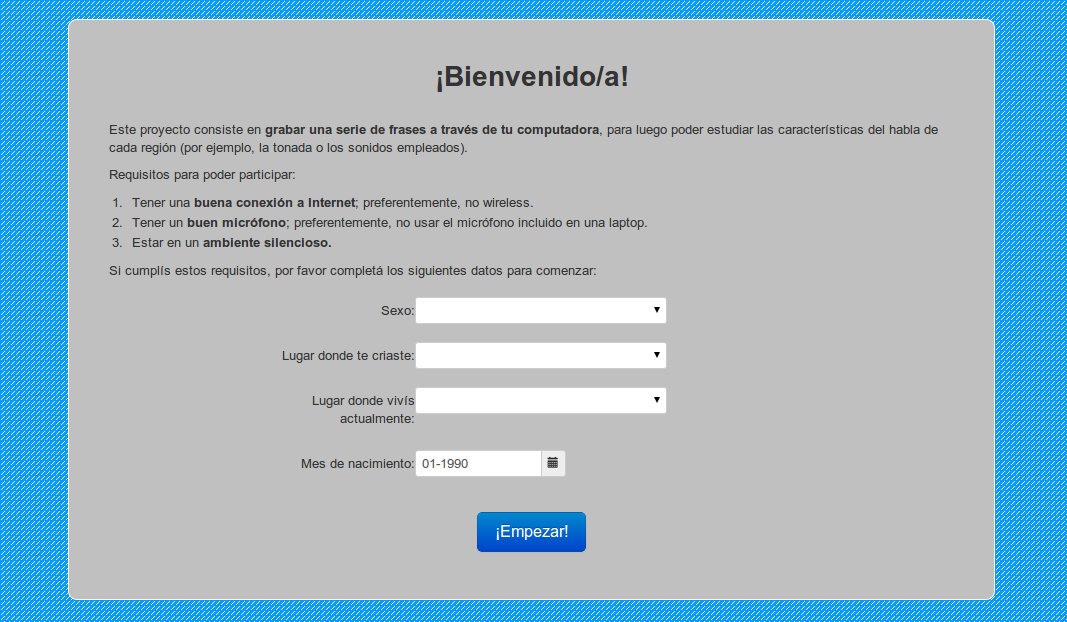
\includegraphics[width=0.8\textwidth]{pag-inicio2} }
    \caption{Encuesta inicial del sistema}
    \label{figEncuesta}
\end{figure}

\begin{figure}[h!]
    \centerline{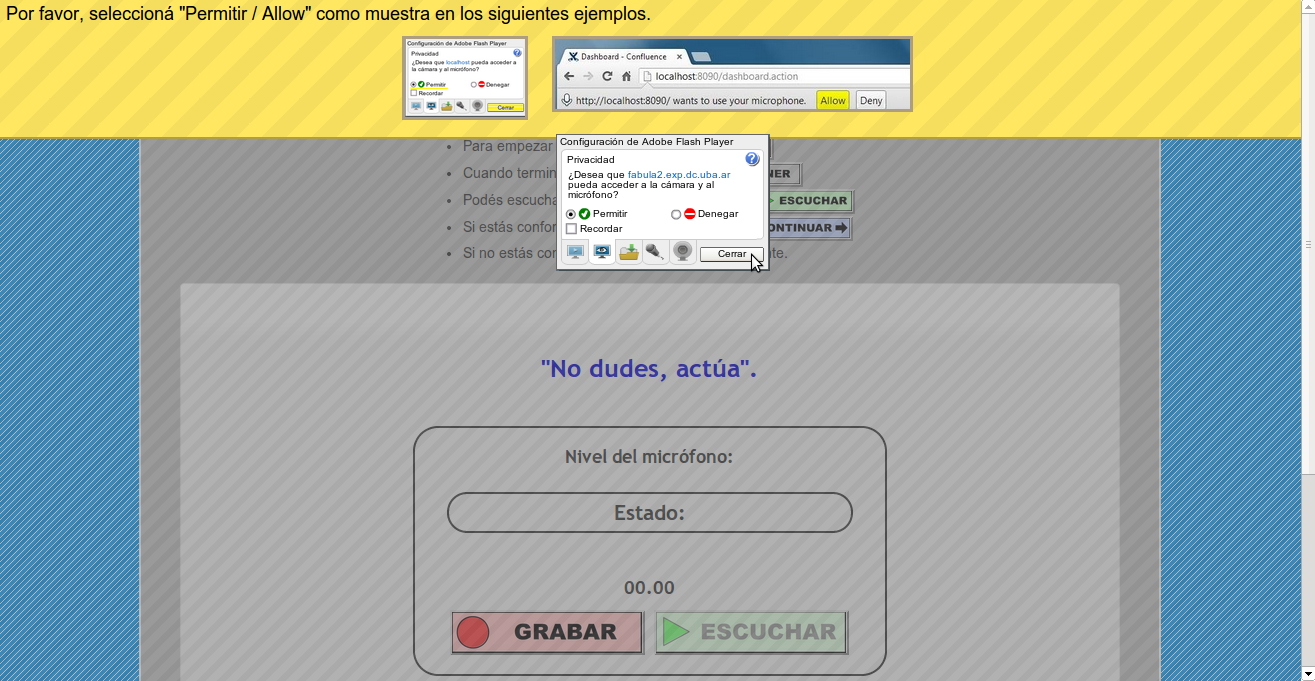
\includegraphics[width=0.8\textwidth]{pag-allow1} }
    \caption{Se debe permitir micrófono para comenzar el experimento}
    \label{allowmic}
\end{figure}

\begin{figure}[h!]
    \centerline{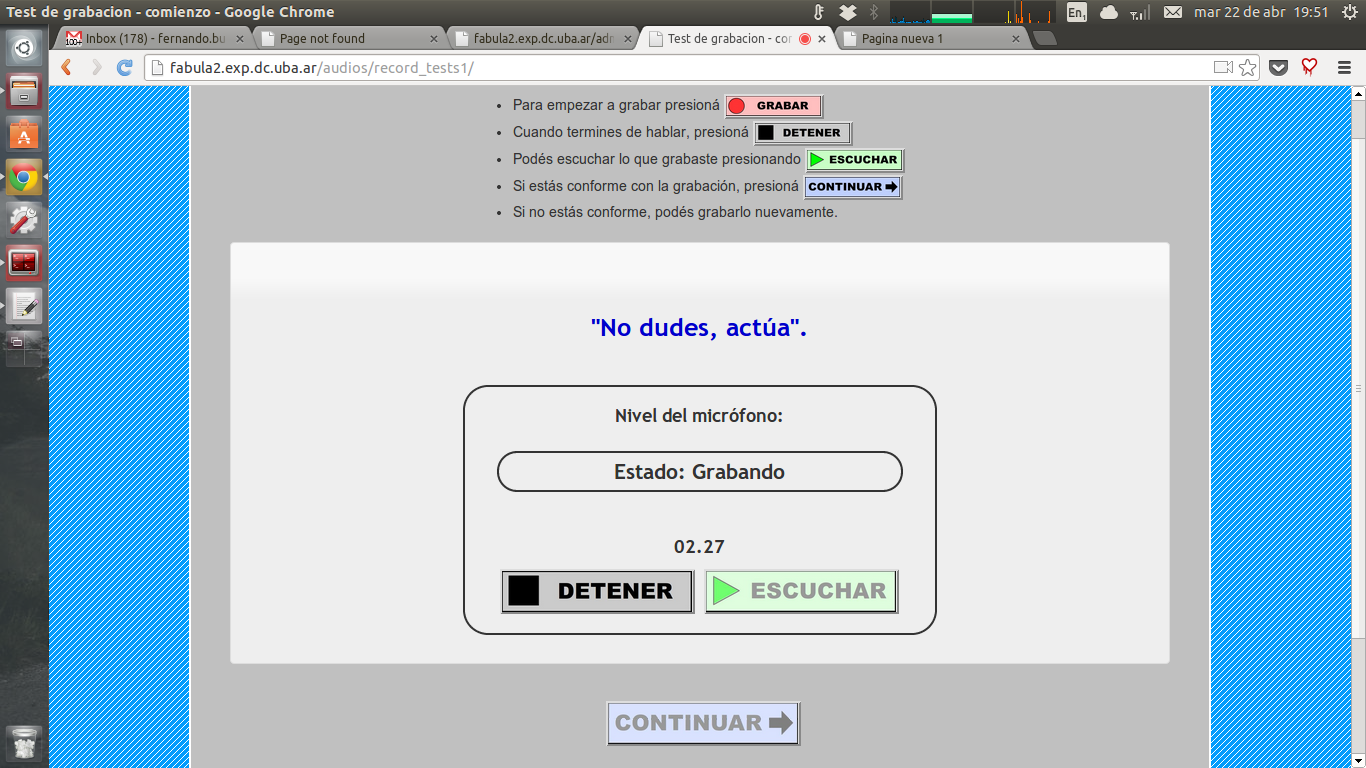
\includegraphics[width=0.8\textwidth]{pag-grabar1} }
    \caption{Grabando una frase}
    \label{grabando}
\end{figure}

\begin{figure}[h!]
    \centerline{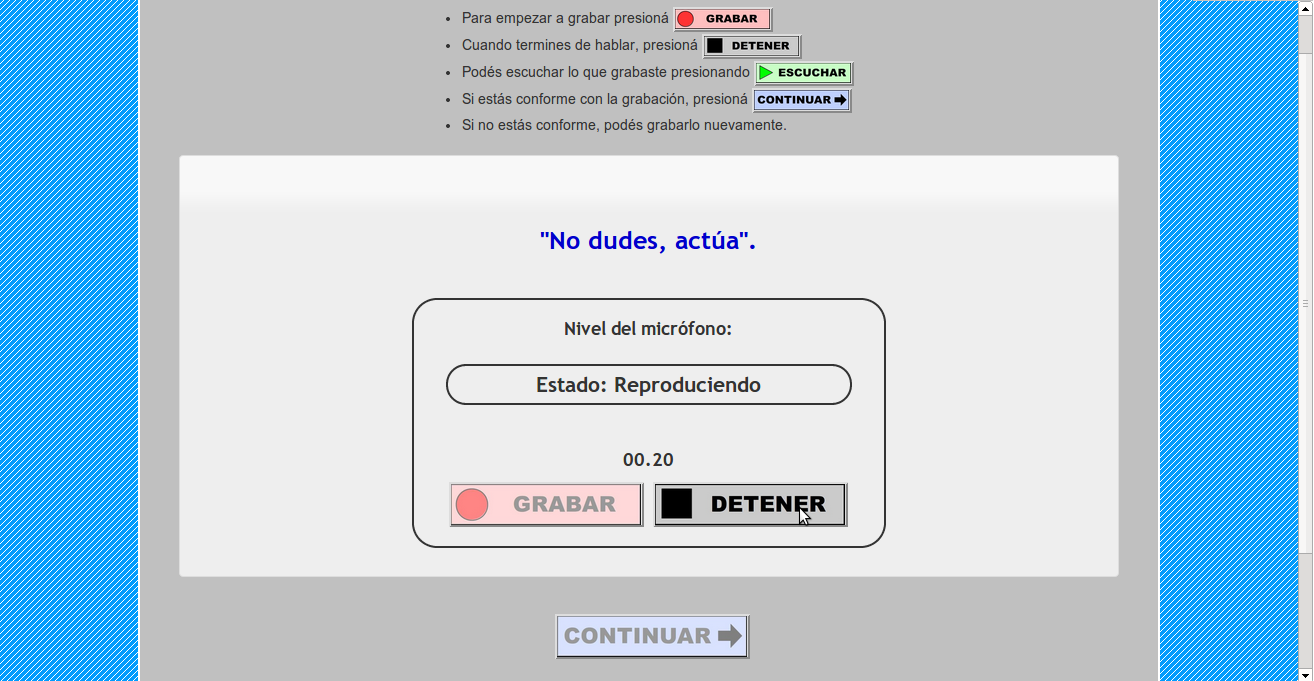
\includegraphics[width=0.8\textwidth]{pag-play1} }
    \caption{Reproduciendo la frase anteriormente grabada}
    \label{reproduciendo}
\end{figure}

En la pantalla de grabación el usuario debe confirmar el acceso al micrófono que posee en su computadora, como se puede apreciar en la Figura \ref{allowmic}. Una vez hecho esto, se le explica las instrucciones del experimento y luego puede empezar a grabar. 

Cada nuevo experimento utiliza una nueva traza del conjunto de trazas descriptas en el capítulo anterior. La interfaz que ve el usuario al grabar cada frase se puede ver en la Figura \ref{grabando}. Las grabaciones pueden ser escuchadas por el usuario. Si el usuario al escucharla nota que no es una buena grabación, tiene la posibilidad de grabarla otra vez. Lo importante es que la última grabación se escuche lo mejor posible. Para que el usuario reproduzca su grabación se aprieta el botón \textit{Reproducir} como se ve en la figura \ref{reproduciendo}. 

Una vez que el hablante cree que su grabación se escuche bien, la confirma. Cada vez que se graba un audio, este se guarda en un archivo wav en el servidor. El archivo que se genera tiene una frecuencia de muestreo de 22050 Hz\footnote{Necesitamos una frecuencia de muestreo que permita analizar las diferencias de los dos grupos sin ocupar excesivo espacio por cada grabación. Elegimos 22,05 KHz ya que nos permite realizar el experimento. Esta frecuencia de muestreo equivale a la mitad de frecuencia de un CD de audio. }, cada muestra se analiza con 16 bits y posee un solo canal. Con estas características pudimos obtener un audio de buena calidad para el experimento que realizamos.

Recordemos que los hablantes graban en series de 5 frases. Una vez terminadas estas 5 frases se le pregunta si querría seguir grabando o terminar el experimento. De esta forma, el hablante aporta el tiempo que puede disponer.

\section{Grabación a través del browser}

Los navegadores actuales no permiten acceder al micrófono directamente. Actualmente está en desarrollo HTML5, tecnología que permitirá acceder al micrófono y a recursos similares de forma más fácil. No se eligió basarse en éste porque sólo los browsers más nuevos lo soportan. Al ser un estándar muy nuevo necesita que el usuario tenga instalada últimas versiones de software y utilizarlo hubiera excluido mucha gente. Teniendo en cuenta esto debimos utilizar una tecnología alternativa. 

Encontramos un proyecto llamado Web Accessible Multimodal Interfaces \footnote{Página web: https://code.google.com/p/wami/} (WAMI). WAMI es una aplicación Flash que nos permite acceder al micrófono a través de JavaScript. Éste es muy utilizado en proyectos similares de procesamiento de habla. Esta herramienta nos permite definir dos URLs importantes: una que se utilizará para enviar el audio grabado y otra para escucharlo.  

Cuando termina de grabar, se envía un mensaje POST al servidor a la URL configurada. El servidor obtiene el paquete de información y lo guarda como archivo wav. Cuando se quiere reproducir algún audio se envía un mensaje GET a la otra URL. El servidor lo responde con el audio requerido y se reproduce en el navegador. También con WAMI se puede configurar la calidad del audio grabado y analizar el nivel del volumen que posee. La biblioteca posee funciones que permiten saber qué nivel de volumen se encuentra en un preciso instante.

\subsection{Requerimientos}

Los requerimientos para participar del experimento son básicos: se debe disponer de micrófono y conexión a Internet. Tuvimos problemas con el browser que se utilizaba: WAMI necesita Flash versión 11.04 que no se encuentra en los repositorios tradicionales de Ubuntu. De esta manera, los navegadores que utilicen Flash instalado por el sistema operativo Ubuntu no podrán correr. Otros sistemas operativos como Windows o MacOS no tienen problemas con la versión de Flash instalada. De todas formas el navegador Chrome posee preinstalado la última versión de Flash, con lo cual este navegador puede correr perfectamente la aplicación sin importar el sistema operativo que se utilice.

\section{Varias grabaciones por frase}

Recordemos que para tener la mejor grabación de cada frase, le dimos la opción al hablante de que pueda escuchar como quedó. Esto requiere un ida y vuelta de paquetes entre el cliente (navegador) y el servidor. 

Al grabar el cliente manda un mensaje al servidor con el audio de la grabación en crudo. La longitud de este paquete tiene un tamaño pequeño ya que las frases son de corta duración. Cuando el cliente quiere escucharlo envía un mensaje pidiendo ese mismo audio anteriormente grabado. El servidor envía el audio y es reproducido en el cliente. Este ida y vuelta de la grabación podría ser optimizada para que la grabación pueda ser escuchada sin tener interacción con el servidor. En nuestro experimento, no tuvimos problemas graves en lo que respecta al tiempo de retardo pero podría ser un punto débil del sistema que hay que tener en cuenta.

Puede resultar interesante analizar las anteriores grabaciones para ver por qué el hablante elige el último. Esta idea también puede motivar a algún trabajo futuro.

\section{Sistema de administración}

Además de la interfaz pública para grabar, implementamos un sistema privado para administrar las grabaciones. Éste nos permite ver las grabaciones que fueron grabadas, la cantidad de grabaciones por cada frase que tenemos recolectada, la cantidad de trazas que todavía no se utilizaron, entre otras cosas. También nos permite escuchar y marcar las grabaciones para utilizarlas como primer filtro de las grabaciones. Explicaremos esto en más detalle a continuación.

\subsection{Etiquetado de audio}

Cuando varias personas terminan el experimento, los administradores pueden acceder a una página donde se puede escuchar cada audio que se va grabando. Los administradores escuchan las grabaciones y según su calidad los etiquetan con alguna de las etiquetas definidas. Las etiquetadas utilizadas esta vez son: `Conservar’,  `Sonido saturado’, `Mucho ruido de fondo’, `Problemas en el habla’. Esto se puede ver en Figura \ref{cat}.

\begin{figure}[h!]
    \centerline{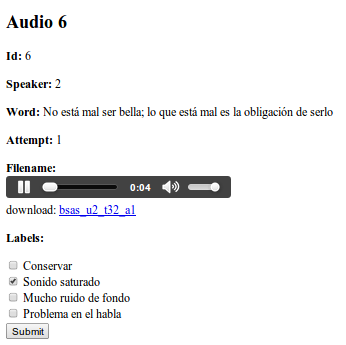
\includegraphics[width=0.5\textwidth]{categorizando_audios} }
    \caption{Categorizando audios}
    \label{cat}
\end{figure}

Para acceder a los audios que fueron etiquetados de una determinada manera, el sistema tiene distintas URLs que nos permiten bajar todos esos audios en un archivo comprimido. Entonces si quisiéramos bajar todo el audio etiquetado con la categoría `Conservar’ podemos acceder a una URL y bajarnos sin necesidad de conectarse al servidor. Se necesita ser usuario del sistema para poder acceder a estas opciones.

\section{Backups automáticos}

El sistema posee backups que se generan a la noche automáticamente. Los backups consisten en un volcado de información de toda la base de datos y en la sincronización de las grabaciones con una carpeta externa de backup.

\section{Análisis del volumen}

Un requerimiento primordial de este experimento es evitar grabaciones saturadas. Para ello medimos el volumen de la grabación mientras ésta se produce. El resultado es una serie de valores entre 0 a 100. Sobre estos valores calculamos el máximo y el mínimo. Si el primero es mayor a un cierto umbral arbitrario (o sea mayor a 80 por ejemplo) significa que la grabación saturó en algún momento. Si el mínimo es menor a un cierto umbral (o sea menor a 20 por ejemplo) quiere decir que hay mucho ruido ambiente. En cualquiera de los dos casos podemos pedirle al usuario que grabe nuevamente el experimento. De esta forma podemos filtrar grabaciones que no nos servirán para reconocer el acento.

Si bien la característica de filtrar por volumen fue programada, no fue utilizada en este experimento. El motivo fue que queríamos chequear cuán bien funcionaba la herramienta sin filtros y con completa participación de los usuarios. Otro motivo fue la paciencia de los hablantes: puede suceder que no se logre un ambiente beneficioso para grabar y el filtro rechace todas sus grabaciones, perdiendo un posible hablante. También notamos que había grabaciones que fueron rechazadas por el filtrado de volumen pero en realidad eran de buena calidad. Esto no lo queremos como primer experimento del framework. Por eso elegimos aceptar todas las grabaciones.

A continuación veremos cómo utilizamos esta información recolectada para el objetivo del experimento.